\chapter{Proposed solution}
\label{cap:cap3}

% (aproximativ 14 pagini)

% \section{Recomandări conținut}

% Prezentarea proiectării și implementării sistemului/aplicației în funcție de specificul acesteia. Ar trebui incluse doar elementele relevante proiectului dintre cele ce urmează.

% \begin{itemize}
%     \item Reiterarea problemei pe care o rezolvă soluția propusă și a strategiei de rezolvare.
%     \item Idei originale, soluții noi.
%     \item Cerințe ale utilizatorului (en., user requirements): așteptările utilizatorilor finali de la sistemul sau aplicația dezvoltată.
%     \item Arhitectura/Modelarea sistemului: descrierea componentelor principale și a interacțiunilor dintre acestea, e.g., prin scheme bloc.
%     \item Proiectarea propriu-zisă:
%     \begin{itemize}
%         \item diagrame ER pentru baze de date,
%         \item UML pentru proiectele care necesită diverse paradigme complexe și lucru cu clase – diagramele pot fi incluse și în anexe,
%         \item pseudocod pentru algoritmii creați,
%         \item scheme logice pentru cei care dezvoltă în limbaje structurate,
%         \item proiectare cablaj imprimat.
%     \end{itemize}
%     \item Descrierea succintă a elementelor (e.g., claselor) dezvoltate și implementate de absolvent.
%     \item Analiza platformei hardware pe care va fi executată respectiva aplicație și se analizează care abordare în implementare ar fi mai bună pentru respectiva structură.
%     \item Alegerea tehnologiilor și justificarea pe scurt a alegerii.
%     \item Identificarea avantajelor și a dezavantajelor metodei alese.
%     \item Descrierea implementării soluției.
%     \item Prezentarea unor capturi de ecran relevante sau a unor imagini cu soluția dezvoltată, e.g., capturi de ecran cu funcționalități importante din interfața cu utilizatorul, poze cu sistemul fizic dezvoltat.
% \end{itemize}

% \section{Exemple și alte elemente de ajutor}

% \begin{itemize}
%     \item se analizează platforma hardware pe care va fi executată respectiva aplicație și se analizează care abordare în implementare ar fi mai bună pentru respectiva structură
%     \item se stabilesc modulele generale ale aplicației și interacțiunile dintre ele;
%     \item se analizează avantaje și dezavantajele metodei alese;
%     \item se indică limitele în care metoda va funcționa. 
% \end{itemize}

% \textit{Componente software:}
% \begin{itemize}
%     \item proiectarea propriu zisă (diagrame ER pentru baze de date, UML pentru proiectele care necesită diverse paradigme complexe și lucru cu clase – orientat obiect, scheme logice pentru cei care dezvoltă în limbaje structurate etc);
%     \item se stabilește tehnologia aleasă pentru implementare și se justifică alegerea făcută;
%     \item se descriu succint numai clasele dezvoltate și implementate de absolvent cu trimitere la pagina din anexă unde se află codul complet;
% \end{itemize}

% Figurile mai complexe, care nu se văd bine în format A4/portrait, pot fi incluse în anexe și referite normal (vezi Figura \ref{fig:AT} din Anexa \ref{anexa3:func_xyz}).

% \vspace{1em}

% \textit{Componente hardware:}
% \begin{itemize}
%     \item stabilirea componentelor hardware necesare. Exemplu: etaje analogice, display-uri, dispozitive I/O, periferice USB, etc.;
%     \item analiza performanțelor și descrierea perifericelor procesorului/microcontrolerului folosit
%     \item realizarea schemei bloc care să reflecte interconectarea componentelor principale;
%     \item simularea funcționării componentelor hardware (OrCAD, Proteus, simulatoare HDL);
%     \item proiectarea cablajului imprimat (Altium Designer, Eagle).
% \end{itemize}

%  (Figura \ref{fig:BB8})

% \begin{figure}[H]
%     \centering
%     \includegraphics[width=0.3\textwidth]{continut/capitol3/figuri/BB8.png}
%     \caption{BB8\protect\footnotemark}
%     \label{fig:BB8}
% \end{figure}
% \footnotetext{imagine preluată de pe un site web care nu „merită” trecut la bibliografie \url{https://www.pngitem.com/}}


% Ecuația \eqref{eq:sample} este un exemplu foarte simplu de formulă matematică. Ecuațiile vor fi referite prin comanda \LaTeX\ \verb|\eqref{}| din pachetul \verb|amsmath|.

% \begin{equation}
%     \label{eq:multiline_sample}
%     \begin{split}
%         A & = \frac{\pi r^2}{2} \\
%          & = \frac{1}{2} \pi r^2
%     \end{split}
% \end{equation}

% \begin{equation}
%     \label{eq:sample}
%     e^{\pi i} + 1 = 0
% \end{equation}

% În ecuația \eqref{eq:multiline_sample} avem un prim exemplu multiline în care alinierea față de simbolul egal este specificată în codul de generare a ecuației.

% În cazul unui număr mare de ecuații poate fi de dorit folosirea de macrodefiniții pentru a standardiza și urmări mai ușor codul de generare al acestora, evitându-se variații de formă și alte greșeli de redactare.
% Un principal avantaj al utilizării macrodefinițiilor pentru notații este că eventualele modificări pot fi propagate rapid și uniform în întregul document.

% Ecuațiile, definițiile și teoremele se referă în textul lucrării de licență/disertație prefixate: ecuația \eqref{eq:sample}, definiția \ref{def:diploma} sau teorema \ref{thm:equal}, iar aici este o pură întâmplare că au același indice, fiind vorba despre prima ecuație, prima definiție și prima teoremă din Capitolul \ref{cap:cap3}.

% În continuare, definiția \ref{def:diploma} introduce conceptul de „Lucrare de diplomă”. Titlul efectiv este opțional și îl regăsiți în \LaTeX\ între [].

% \begin{definition}[Lucrare de diplomă]
%     \label{def:diploma}
%     Lucrarea de diplomă face dovada nivelului și calității pregătirii profesionale, teoretice și aplicative a absolventului, iar prin modul în care aceasta este prezentată (susținută public în fața unei comisii de examinare) ea evidențiază calitățile științifice și inginerești definitorii ale absolventului.
% \end{definition}

% Numerotarea teoremelor se va face similar ecuațiilor și definițiilor de mai sus. Vezi teorema \ref{thm:equal}.

% \begin{theorem}[Teorema egalității]
%     \label{thm:equal}
%     Dacă $a=b$, atunci $b=a$.
% \end{theorem}

% \begin{proof}
% Ne bazăm pe proprietatea de reflexivitate.
% \end{proof}

% În acest capitol ar trebui să se regăsească un algoritm (dacă este cazul) și el va fi referit ca Algoritmul \ref{alg:acceptance}.

% \begin{algorithm}[ht]
%     \caption{Pseudo code for reviewing process}\label{alg:acceptance}
%     \begin{algorithmic}[1]
%         \Procedure{Acceptance}{paper, committee}
%             \State $\textit{reviewers} \gets \text{randomly select } \{(i,j) \mid i,j \in  \{1, \cdots, \#\{\textit{committee}\}\}, i \neq j \}$
%             \State $\textit{reviews} \gets 2 \times 1 \text{ array of } \textit{False}$
%             \BState \emph{reviewing round}:
%             \For {$i \in \textit{reviewers }$}
%                 \If {$paper \text{ reads well for } \textit{committee}(i) $}
%                     \State $\textit{review}(i) \gets \textit{True}$.
%                 \Else \text{ do nothing}
%                 \EndIf
%             \EndFor
%             \BState \emph{evaluation round}:
%             \If {$\textit{reviews}(i) \text{ is } \textit{False} \text{ for all } i \in \textit{reviewers}$}
%                 \State \textbf{goto} \emph{hell}.
%             \ElsIf {$\textit{reviews}(i) \text{ is } \textit{True} \text{ for all } i \in \textit{reviewers}$}
%                 \State \textbf{goto} \emph{Licența 2022}
%             \Else \textbf{ goto} \emph{revision round}
%             \EndIf
%             \BState \emph{revision round}:
%             \State $\textit{reviser} \gets \text{randomly select } \{i \mid i \in  \{1, \cdots, \#\{\textit{committee}\}\}, i \not\in \textit{reviewers} \}$
%             \If {$paper \text{ reads well for } \textit{committee(reviser)} $}
%                 \State \textbf{ goto} \emph{Licența 2022}
%             \ElsIf{\textit{committee(reviser)} \text{ has no opinion and likes inifinite loop}}
%                 \State \textbf{ goto} \emph{reviewing round}
%             \Else \textbf{ goto} \emph{hell}
%             \EndIf
%             \BState \emph{hell} 
%             \State \text{Try again in summer 2023!}
%             \BState \emph{Licența 2022 (some people also call it hell)}:
%             \State \text{See you at Beer Zone!}
%         \EndProcedure
%     \end{algorithmic}
% \end{algorithm}

% În acest capitol se descrie și implementarea practică a proiectului. În mod uzual, puteți insera cod de dimensiuni mici, care este relevant și care se impune a fi comentat în detaliu. Astfel, Listing-ul \ref{code:c_mpi} prezintă un supergreu pas de inițializare a unui program MPI pentru a obține cinstit punctul din oficiu, în care se poate face referire la linia \ref{line:if} pentru a descrie ce face \verb|if|-u' di acolo.

% \begin{code}
%     \begin{minted}{c}
%         #include <stdio.h>
%         #include "mpi.h"
        
%         int main( int argc, char **argv ) {
%         	char message[20];
%         	int myrank;	
        		
%         	MPI_Status status;
        
%         	MPI_Init( &argc, &argv );
%         	MPI_Comm_rank( MPI_COMM_WORLD, &myrank );
        	
%         	if (myrank == 0) { /* codul pentru procesul 0 */|\label{line:if}|
%         		strcpy(message,"Hello");
%         		MPI_Send(message, strlen(message), MPI_CHAR, 
%         			1, 99, MPI_COMM_WORLD);
%         	} else { /* codul pentru procesul 1 */
%         		MPI_Recv(message, 20, MPI_CHAR, 
%         			0, 99, MPI_COMM_WORLD, &status);
%         		printf("received :%s:\n", message);
%         	}
        	
%         	MPI_Finalize();
%         	return 0;
%         }
%     \end{minted}
%     \caption{Supercod MPI în C} 
%     \label{code:c_mpi}
% \end{code}

% Codul complet relevant se va include în anexe (vezi Anexele \ref{anexa6:listing_python}, \ref{anexa7:listing_kotlin} și \ref{anexa8:listing_xml}). De exemplu, Listing-ul \ref{code:xml_pom} (Anexa \ref{anexa8:listing_xml}) prezintă fișierul de configurare \textit{maven} pentru un serviciu SOAP minimal.

This chapter presents the design and implementation of the experimental solution used to analyze the influence of validation protocols on biomass estimation performance. The chapter begins by restating the problem and the requirements imposed on the experimental pipeline. It then describes the dataset, the preprocessing and feature-extraction stages, the predictive models, the validation protocols, and the evaluation metrics. Finally, the implementation details, reproducibility choices, and limitations of the proposed solution are discussed.

\section{Problem Restatement and Experimental Requirements}

The main research question of this work is not whether a particular model can predict biomass accurately, but whether the validation protocol used during model development provides a realistic estimate of the model's generalization ability on unseen data affected by temporal and spatial shifts.

To answer this question in a controlled manner, the solution must satisfy several requirements.

\textbf{Functional requirements:}
\begin{itemize}
    \item \textbf{FR1:} The pipeline shall load the public CSIRO Image2Biomass dataset, including images and biomass target values.
    \item \textbf{FR2:} The pipeline shall preprocess images consistently for training, validation, and inference.
    \item \textbf{FR3:} The pipeline shall extract visual representations using the DINOv3 ViT-L/16 model in frozen mode.
    \item \textbf{FR4:} The pipeline shall train at least two regression models: a Ridge baseline and a Multi-Layer Perceptron.
    \item \textbf{FR5:} The pipeline shall support Random CV, Date CV, and Date-State CV protocols.
    \item \textbf{FR6:} The pipeline shall compute the local weighted $R^2_w$ metric, RMSE, MAE, and the optimism gap.
    \item \textbf{FR7:} The pipeline shall produce final predictions for the hidden Kaggle test set using test-time augmentation.
\end{itemize}

\textbf{Non-functional requirements:}
\begin{itemize}
    \item \textbf{NFR1 -- Isolation of the validation effect:} All components except the data-splitting strategy shall be kept unchanged across experiments.
    \item \textbf{NFR2 -- Reproducibility:} All stochastic processes shall be controlled through fixed random seeds.
    \item \textbf{NFR3 -- Modularity:} Data loading, preprocessing, feature extraction, model training, validation, and evaluation shall be implemented as separate modules.
    \item \textbf{NFR4 -- Computational efficiency:} Visual embeddings shall be precomputed once and reused across experiments.
\end{itemize}

These requirements ensure that the observed differences between validation protocols can be attributed primarily to the splitting strategy, rather than to changes in model architecture, data processing, or optimization settings.

\section{Solution Overview and Architecture}

The proposed solution is organized as a modular experimental pipeline. Before presenting the architecture, it is useful to describe the main design choices that motivate the structure shown in Figure~\ref{fig:model_overview}.

Each original image has a resolution of $2000 \times 1000$ pixels and represents a pasture quadrat. Because the image is much wider than tall, the left and right halves are treated as two separate views of the same plot. This decision preserves spatial detail while producing square inputs compatible with the DINOv3 ViT-L/16 architecture. Applying independent augmentations to each half during training acts as a form of regularization and greatly increases the number of augmented views available to the model. Although this means that the two halves of the same image can receive different transformations, this is intentional: it encourages the model to rely on stable visual patterns rather than on image orientation or illumination.

\begin{figure}[t]
    \centering
    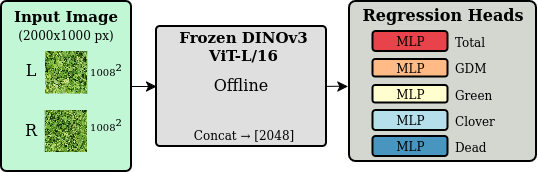
\includegraphics[width=0.8\textwidth]{continut/capitol3/figuri/fig_pipeline_overview.png}
    \caption{Overview of the preprocessing, embedding extraction, and multi-branch regression pipeline used in all experiments.}
    \label{fig:model_overview}
\end{figure}

The pipeline consists of five main stages:

\begin{enumerate}
    \item \textbf{Data ingestion:} The public dataset is loaded, metadata are parsed, and images are associated with their five biomass target values.
    \item \textbf{Preprocessing and augmentation:} Each image is split into two halves, resized, and augmented according to the stage of the experiment.
    \item \textbf{Feature extraction:} The DINOv3 ViT-L/16 backbone is used in frozen mode to compute visual embeddings.
    \item \textbf{Model training and local validation:} Ridge and MLP models are trained under multiple validation protocols on the computed embeddings.
    \item \textbf{Inference and submission:} Final models are retrained on the full public dataset and used to generate hidden-test predictions through test-time augmentation.
\end{enumerate}

This separation makes it possible to run systematic experiments without altering the core prediction pipeline.

\section{The Dataset Used}

The study uses the CSIRO Image2Biomass dataset introduced by Liao et al.~\cite{liao2025estimating}. The public split contains 357 top-view pasture images collected in 2015 from 19 locations across four Australian states.

\begin{table}[htbp]
\centering
\caption{Descriptive statistics of the five biomass targets in the public split.}
\label{tab:dataset_stats}
\small

\begin{threeparttable}
\begin{tabular}{lccccc}
\hline
\textbf{Variable} & \textbf{Mean} & \textbf{Std} & \textbf{Min} & \textbf{Median} & \textbf{Max} \\
\hline
Dry\_Green & 26.62 & 25.4 & 0 & 20.8 & 157.98 \\
Dry\_Dead & 12.04 & 12.4 & 0 & 7.98 & 83.84 \\
Dry\_Clover & 6.65 & 12.12 & 0 & 1.42 & 71.79 \\
GDM & 33.27 & 24.94 & 1.04 & 27.11 & 157.98 \\
Dry\_Total & 45.32 & 27.98 & 1.04 & 40.3 & 185.7 \\
\hline
\end{tabular}

\end{threeparttable}
\end{table}

Each image represents a pasture quadrat of size $70\,\text{cm} \times 30\,\text{cm}$. The associated labels are five dry biomass components measured in grams per quadrat:

\begin{table}[htbp]
\centering
\caption{Biomass target variables and their weights in the official competition metric.}
\label{tab:target_variables}
\begin{tabular}{lcc}
\hline
\textbf{Variable} & \textbf{Weight in $R^2_w$} & \textbf{Description} \\
\hline
Dry\_Green  & 0.1 & Dry weight of green vegetation \\
Dry\_Dead   & 0.1 & Dry weight of dead vegetation \\
Dry\_Clover & 0.1 & Dry weight of clover \\
GDM         & 0.2 & Green dry matter component \\
Dry\_Total  & 0.5 & Total dry biomass \\
\hline
\end{tabular}
\end{table}

The dataset is particularly suitable for studying validation effects because it contains strong temporal and spatial structure. Images were collected during several campaigns in 2015, meaning that many observations share the same acquisition date, location, weather conditions, and sensor settings. The hidden test set, by contrast, contains more than 800 images from 2014 and 2016 and does not provide metadata. Therefore, local validation on the 2015 public data may not fully represent the distribution encountered in hidden evaluation.

Figure~\ref{fig:dataset_overview} provides an overview of the public split, including example imagery, target distributions, and acquisition dates.

\begin{figure*}[t]
    \centering
    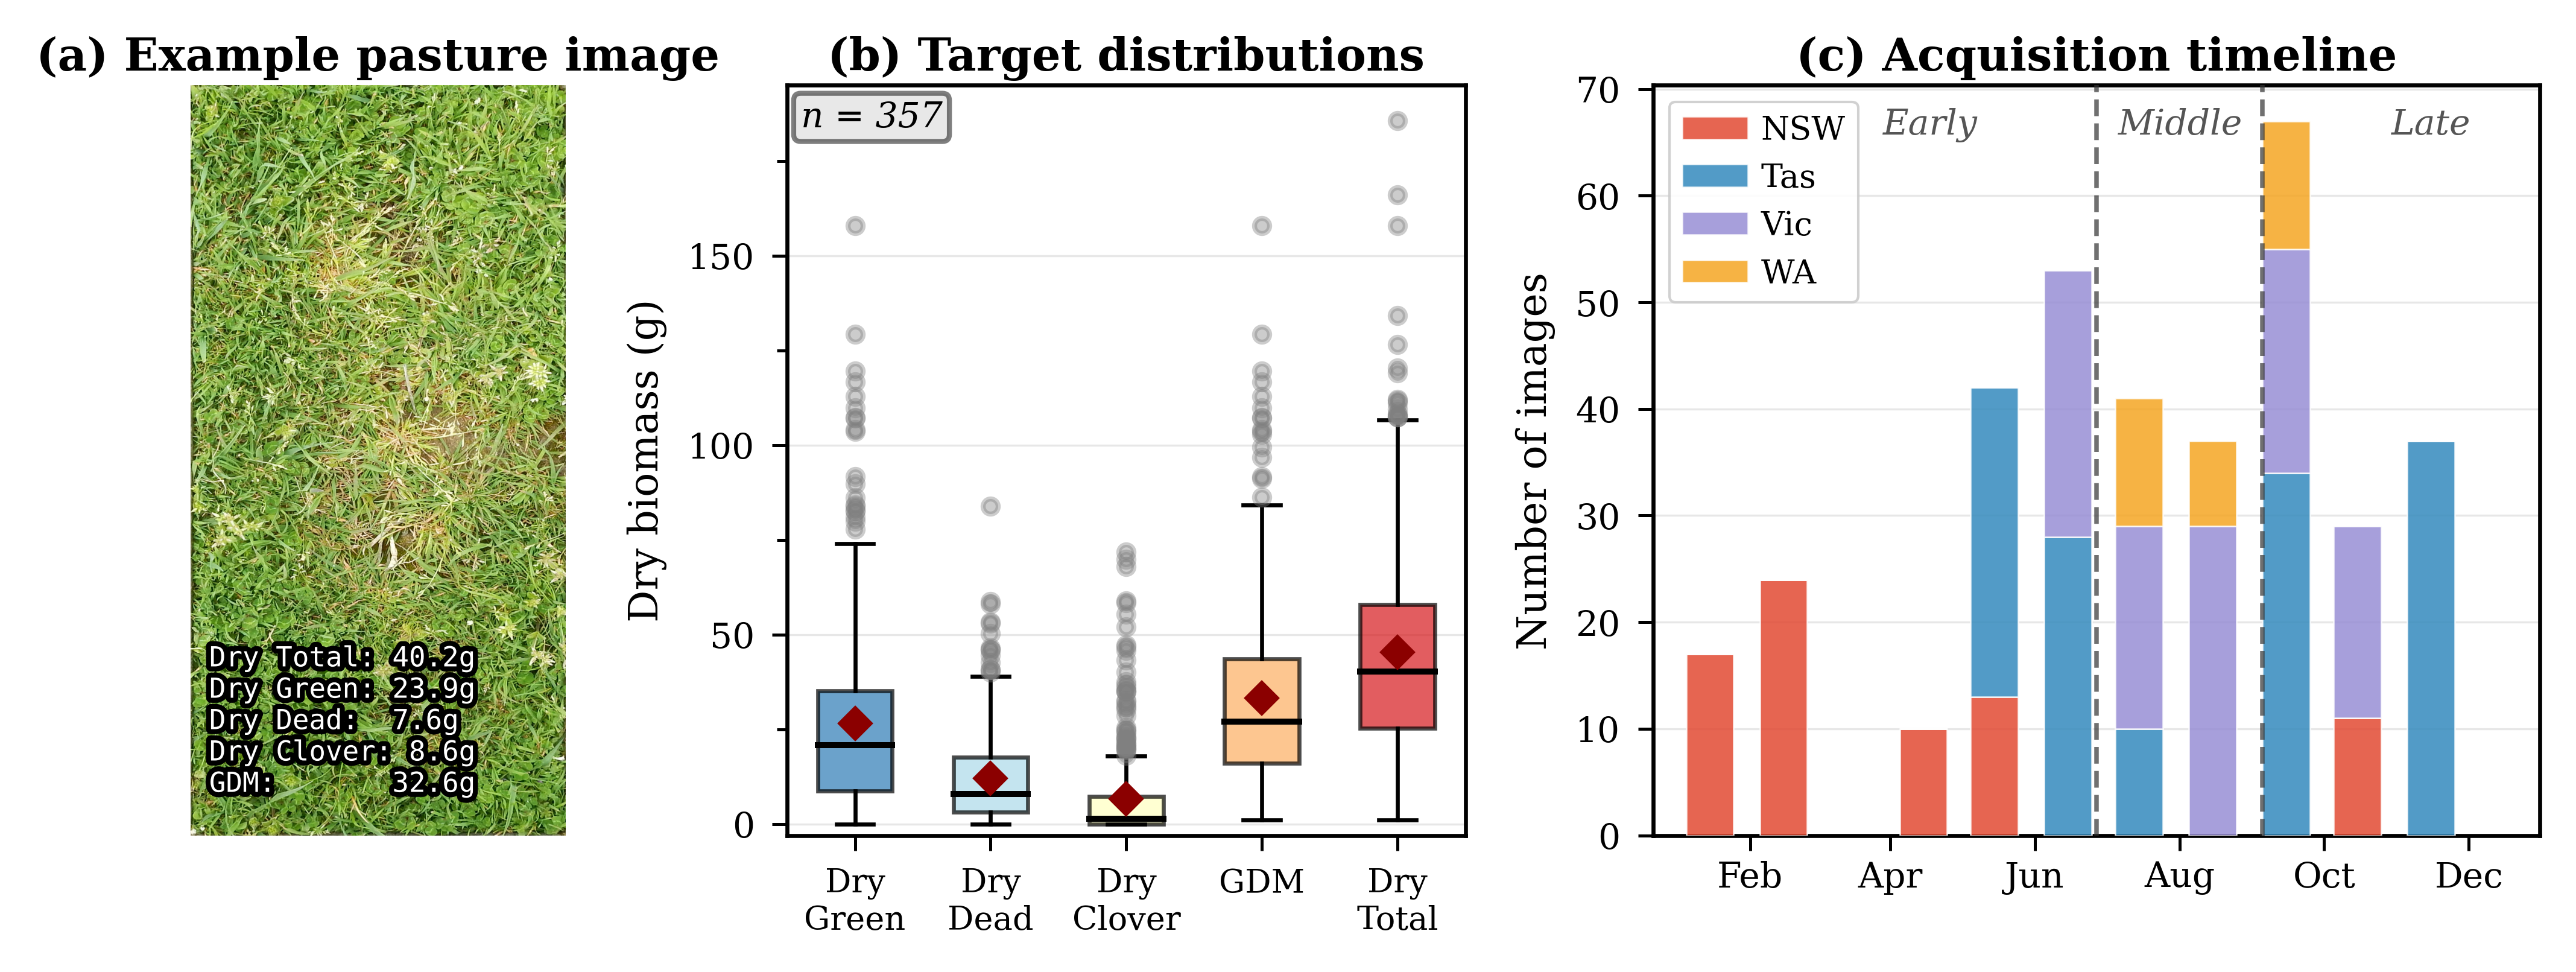
\includegraphics[width=\textwidth]{continut/capitol3/figuri/fig_dataset_overview.png}
    \caption{
    Overview of the CSIRO Image2Biomass public split.
    (a) Example top‑view pasture quadrat (70\,cm $\times$ 30\,cm).
    (b) Distributions of the five dry‑weight biomass targets ($g$ per quadrat).
    (c) Temporal distribution of image acquisitions in 2015, coloured by Australian state.
    Vertical dashed lines indicate the early/middle/late temporal blocks used in the LOPO analysis.
    }
    \label{fig:dataset_overview}
\end{figure*}

\section{Preprocessing and Augmentation Pipeline}

All images are preprocessed in the same way before being passed to the feature extractor.

Each original image has a resolution of $2000 \times 1000$ pixels. The image is first split into two square halves, left and right. Each half is then resized to $1008 \times 1008$ pixels. This operation preserves spatial detail while producing square inputs compatible with the ViT-L/16 architecture.

During training, spatial and photometric augmentations are applied independently to each half:

\begin{itemize}
    \item horizontal flip;
    \item vertical flip;
    \item rotation by $90^\circ$;
    \item color jitter with brightness, contrast, and saturation set to $0.5$, and hue set to $0.05$.
\end{itemize}

After augmentation, both halves are normalized using ImageNet statistics. During validation and final inference, only resizing and normalization are applied.

Table~\ref{tab:preprocessing} summarizes the preprocessing and augmentation choices.

\begin{table}[htbp]
\centering
\caption{Preprocessing and augmentation configuration.}
\label{tab:preprocessing}
\begin{tabular}{ll}
\hline
\textbf{Stage} & \textbf{Configuration} \\
\hline
Original resolution & $2000 \times 1000$ \\
Splitting & Left and right halves \\
Resize & $1008 \times 1008$ \\
Training spatial augmentation & H/V flips, $90^\circ$ rotations \\
Training photometric augmentation & Brightness, contrast, saturation $=0.5$; hue $=0.05$ \\
Normalization & ImageNet mean and standard deviation \\
Validation/inference & Resize and normalization only \\
\hline
\end{tabular}
\end{table}

As explained earlier in this chapter, the augmentation strategy was selected to improve local robustness without introducing excessive distribution shift. By applying photometric and geometric transformations, the model is encouraged to rely on stable visual patterns rather than on image orientation or illumination.

\section{Feature Extraction with DINOv3}

Visual features are extracted using the DINOv3 ViT-L/16 model~\cite{simeoni2025dinov3} in frozen mode. This means that the backbone weights are kept fixed and no gradients are propagated through the feature extractor during model training.

For each image half, multiple augmented views are generated. Each view is passed through the DINOv3 backbone, producing an embedding of dimension $1024$. The embeddings corresponding to the two halves are concatenated, resulting in a final feature vector of dimension $2048$.

All embeddings are precomputed and stored on disk. This design choice separates feature extraction from model training and reduces computational cost. For the Ridge baseline, only the original non-augmented embeddings are used for training and validation. For the MLP model, 15 augmented embeddings are generated per image half, together with the original-augmentation embedding. During MLP training, one embedding per image is randomly sampled from the available set at each step. Validation is always performed using only the original embedding.

At final inference, test-time augmentation uses five fixed views: the original image, horizontal flip, vertical flip, $180^\circ$ rotation, and transpose. All augmented views derived from the same original image are assigned to the same cross-validation fold, so no view of a validation image is used in training.

Using a frozen feature extractor is essential for this study. It isolates the effect of the validation protocol from the effect of representation learning. If the backbone were fine-tuned, the model could adapt to the public data distribution and introduce an additional source of variation that would be difficult to separate from the validation effect.

\section{Regression Models}

Two regression models are used: a Multi-Layer Perceptron and a Ridge regression baseline. Both models receive the same $2048$-dimensional feature vector and predict the five target variables.

\subsection{Multi-Layer Perceptron Model}

The MLP model consists of five independent branches. Each branch receives the same shared input representation and produces the prediction for one biomass component: \textit{Dry\_Total}, \textit{GDM}, \textit{Dry\_Green}, \textit{Dry\_Clover}, and \textit{Dry\_Dead}, previously shown in Table \ref{tab:target_variables}.

Each branch has the following architecture:

\[ \begin{aligned} \text{Input}(2048) &\rightarrow \text{Linear}(2048,1024) \rightarrow \text{GELU} \rightarrow \text{Dropout}(p=0.3) \\ &\rightarrow \text{Linear}(1024,512) \rightarrow \text{GELU} \rightarrow \text{Dropout}(p=0.3) \\ &\rightarrow \text{Linear}(512,1) \rightarrow \text{Softplus} \end{aligned} \]

The Softplus activation ensures non-negative predictions, which is appropriate for biomass quantities. The multi-branch design allows each target to have a separate head while sharing the same visual representation.

The model is trained using the AdamW optimizer~\cite{loshchilov2017decoupled} with the configuration shown in Table~\ref{tab:training_config}.

\begin{table}[htbp]
\centering
\caption{MLP training configuration.}
\label{tab:training_config}
\begin{tabular}{ll}
\hline
\textbf{Hyperparameter} & \textbf{Value} \\
\hline
Optimizer & AdamW \\
Learning rate & $1 \times 10^{-3}$ \\
Weight decay & $1 \times 10^{-2}$ \\
Batch size & 8 \\
Maximum epochs & 80 \\
Early stopping patience & 15 epochs \\
Loss function & Weighted mean squared error \\
Validation metric & $R^2_w$ \\
\hline
\end{tabular}
\end{table}

The hyperparameters were selected through manual trial and error, guided by general practices and by observing training behaviour. The goal was not to maximize absolute performance, but to obtain a stable and reproducible model that behaves consistently across all validation protocols. For this reason, no systematic hyperparameter search or fine-tuning was performed.

The learning rate, weight decay, and dropout values were found to produce stable validation curves without excessive overfitting. The maximum number of epochs and the early stopping patience were set large enough to allow convergence under the more difficult grouped protocols, but not so large as to encourage unnecessary overfitting.

The batch size of 8 was retained from the original competition setup. Since the visual embeddings are precomputed and the MLP is very small, larger batch sizes would have been computationally feasible. The batch size was not systematically tuned because the chosen value already produced stable training behaviour across all validation protocols.

The loss function is the weighted mean squared error:

\[
\mathcal{L}_{\text{WMSE}} =
\frac{1}{N}
\sum_{i=1}^{N}
\sum_{j=1}^{5}
w_j \left(y_{ij} - \hat{y}_{ij}\right)^2,
\]

where $w_j$ are the official competition weights. This loss function follows the weighting scheme of the competition metric but is easier to optimize directly than $R^2_w$.

Early stopping is performed using the local validation $R^2_w$. The best epoch is selected for each fold and each seed.

\subsection{Ridge Baseline Model}

A Ridge regression model is used as a simple linear baseline. The Ridge model is wrapped in the \texttt{MultiOutputRegressor} class from Scikit-Learn, meaning that one Ridge regressor is fitted for each of the five targets.

The regularization parameter is selected using \texttt{RidgeCV} over the following candidate values:

\[
\alpha \in \{10^{-3}, 10^{-2}, 10^{-1}, 1, 10, 100, 1000\}.
\]

These values cover a wide logarithmic range and are sufficient to observe whether regularization strength has a meaningful effect on the linear baseline.

The Ridge model is trained exclusively on the clean, original embeddings without any augmented views. During validation and final inference, predictions are obtained from the clean embeddings only. Test-time augmentation is not used for Ridge, because the model is trained only on clean embeddings and the augmented views would differ from the training distribution.

The Ridge model uses the same validation folds as the MLP. It has no hidden layers, no early stopping, and no additional nonlinear transformations.

The purpose of the Ridge baseline is to test whether the observed differences between validation protocols depend on model complexity. If similar trends appear for both Ridge and MLP, the effect can be attributed mainly to the validation strategy.

\section{Validation Protocol Design}

The central component of the proposed solution is the validation protocol layer. Three protocols are implemented.

For all protocols, five-fold cross-validation is used. Each protocol is repeated for five different random seeds. Thus, each protocol produces $5 \times 5 = 25$ runs. Local results are reported as the mean and standard deviation over these runs.

Stratification is performed using five intervals of the \textit{Dry\_Total} variable. This variable was selected because it has the largest weight in the official metric and provides a meaningful summary of total biomass.

The first protocol, Random CV, splits the dataset using stratified five-fold cross-validation without any temporal or geographic constraints. This is the standard validation procedure used in many machine learning studies. Because images from the same collection campaign can appear in different folds, Random CV tends to overestimate performance when the data contain temporal or spatial dependencies.

The second protocol, Date CV, treats all images collected on the same day as an indivisible group. The folds are constructed so that no group is split across training and validation. This constraint prevents the model from seeing images acquired on the same day as the validation images, thereby reducing temporal leakage.

The third protocol, Date-State CV, groups together images that share the same acquisition date and the same Australian state. These groups are then used as the basic units for fold construction. This protocol introduces a stricter grouping constraint than Date CV and is intended to capture both temporal and spatial structure in the data.

\subsection{Final Model Selection and Hidden-Test Evaluation}

For each validation protocol, the optimal stopping epoch is determined as the median of the best epochs across the 25 runs.

The final model is then retrained from scratch on the entire public dataset using the training duration determined for that protocol. During inference, test-time augmentation is applied using five variants:

\begin{itemize}
    \item original image;
    \item horizontal flip;
    \item vertical flip;
    \item $180^\circ$ rotation;
    \item transpose.
\end{itemize}

The predictions from these five variants are averaged to produce the final output. For each random seed, a separate submission is made to the Kaggle platform. The final hidden-test performance is calculated as the mean score over all seeds.

This procedure applies to the MLP model, because its final weights depend on the random initialization and on the randomly sampled augmented embeddings during training. For the Ridge model, the final weights are deterministic after hyperparameter selection and use of the original embeddings. Therefore, a single final Ridge submission is generated and evaluated once.

This procedure ensures that the hidden test set is never used for model selection or early stopping. The only information obtained from the hidden evaluation is the final metric value.

\begin{algorithm}[ht] 
\caption{Grouped cross-validation evaluation protocol} 
\begin{algorithmic}[1] 
\Require Metadata, split strategy, model head, seeds S, folds K=5 
\For{each seed $s \in S$}
\State Construct grouped stratified folds using the selected strategy 
\For{each fold k} 
\State Create training and validation image sets 
\If{head = MLP}
\State Train using mini-batch optimization 
\State Evaluate on validation set after each epoch 
\State Keep predictions from epoch with highest validation weighted $R^2$ 
\State Apply early stopping 
\Else 
\State Fit Ridge regression on training embeddings 
\State Predict validation targets 
\EndIf 
\State Store fold predictions and targets 
\EndFor 
\State Aggregate fold predictions into out-of-fold predictions 
\State Compute overall weighted $R^2$ for seed s 
\EndFor 
\State Report mean and standard deviation of out-of-fold weighted $R^2$ across seeds \end{algorithmic} 
\end{algorithm}

\subsection{LOPO Exploratory Analysis}

As an additional robustness analysis, a Leave-One-Period-Out procedure is used. The 2015 public data are divided into three consecutive temporal blocks:

\begin{itemize}
    \item early period: January 15 -- June 26, 130 images;
    \item middle period: June 29 -- September 4, 131 images;
    \item late period: September 11 -- November 10, 96 images.
\end{itemize}

Each period is removed in turn and used exclusively for testing while the model is trained on the remaining periods.

The LOPO analysis is exploratory and is not used as a primary evaluation protocol. It provides a stricter temporal separation than standard cross-validation and helps reveal whether the difficulty of generalization is uniform within the 2015 data.

\section{Evaluation Metrics}

The primary evaluation metric is the global weighted coefficient of determination $R^2_w$, identical to the official metric used in the Kaggle competition.

Let $\hat{\mathbf{y}} \in \mathbb{R}^{N \times 5}$ be the matrix of predictions and $\mathbf{y} \in \mathbb{R}^{N \times 5}$ the matrix of true values. The weight vector is:

\[
\mathbf{w} = [0.1, 0.1, 0.1, 0.2, 0.5],
\]

corresponding to \textit{Dry\_Green}, \textit{Dry\_Dead}, \textit{Dry\_Clover}, \textit{GDM}, and \textit{Dry\_Total}.

The global weighted mean is computed as:

\[
\bar{y}_w =
\frac{\sum_{i,j} w_j y_{ij}}
     {\sum_{i,j} w_j}.
\]

The residual sum of squares and total sum of squares are:

\[
SS_{\text{res}} =
\sum_{i,j} w_j (y_{ij} - \hat{y}_{ij})^2,
\qquad
SS_{\text{tot}} =
\sum_{i,j} w_j (y_{ij} - \bar{y}_w)^2.
\]

The weighted coefficient of determination is:

\[
R^2_w =
1 - \frac{SS_{\text{res}}}{SS_{\text{tot}}}.
\]

In addition to $R^2_w$, RMSE and MAE are reported. For the LOPO analysis, the bias for \textit{Dry\_Total} is also calculated to identify systematic overestimation or underestimation.

To quantify validation optimism, the optimism gap is defined as:

\[
\Delta_{\text{hidden}} =
R^2_{\text{local}} - R^2_{\text{hidden}},
\]

where $R^2_{\text{local}}$ represents the performance estimated through local validation (calculated using the out-of-fold predictions), and $R^2_{\text{hidden}}$ represents the performance obtained on the competition's hidden test set. Higher values of $\Delta_{\text{hidden}}$ indicate a more pronounced overestimation of the actual performance and, implicitly, a higher degree of optimism of the validation protocol used.

Unlike $R^2_w$, there is no universally accepted threshold for interpreting $\Delta_{\text{hidden}}$. Values close to zero indicate that local validation provides a realistic estimate of generalization performance, whereas larger values indicate increasing optimism. For this reason, the metric is primarily used in a comparative manner. The relative reduction in $\Delta_{\text{hidden}}$ between two validation protocols quantifies how much the discrepancy between local and hidden-test performance has been reduced and therefore how much more reliable the validation estimate becomes.

\section{Implementation Details and Reproducibility}

The implementation was carried out in Python using the following main libraries:

\begin{itemize}
    \item \textbf{PyTorch} for developing and training the MLP model;
    \item \textbf{Scikit-Learn} for Ridge regression, cross-validation, and metric computation;
    \item \textbf{NumPy} and \textbf{Pandas} for data manipulation;
    \item \textbf{Matplotlib} and \textbf{Seaborn} for visualization;
    \item \textbf{Kaggle} for hidden-test evaluation.
\end{itemize}

The code is organized into several modules:

\begin{itemize}
    \item \texttt{data/}: dataset loading, augmentation, preprocessing;
    \item \texttt{evaluation/}: metric computation and local model evaluator;
    \item \texttt{inference/}: feature extractor, tta transforms, submission generation;
    \item \texttt{models/}: Ridge and MLP implementations;
    \item \texttt{training/}: model trainer, loss functions;
    \item \texttt{utils/}: helper functions;
    \item \texttt{scripts/}: cross-validation training, inference scripts.
\end{itemize}

Reproducibility is enforced through fixed random seeds for all stochastic operations. The same seeds are used across all protocols, ensuring that differences are not caused by random initialization or data shuffling.

Several data-leakage controls are implemented. No test fold is used during training or early stopping. For each fold, the validation predictions are obtained only from a model trained on the remaining folds. The hidden test set is used exclusively for final scoring and is never inspected during model development.


\section{Design Advantages, Disadvantages, and Scope}

The proposed design has several advantages:

\begin{itemize}
    \item The frozen DINOv3 feature extractor isolates the effect of the validation protocol from representation learning.
    \item The Ridge baseline provides a simple reference that helps distinguish validation effects from model-specific behavior.
    \item Multiple random seeds reduce the influence of stochastic variation.
    \item The grouped validation protocols simulate temporal and spatiotemporal dependencies.
    \item Precomputed embeddings reduce computational cost and make systematic experimentation feasible.
\end{itemize}

The design also has limitations:

\begin{itemize}
    \item The use of a frozen backbone may limit absolute predictive performance compared with fine-tuned models.
    \item The public dataset is small and comes from a single year, which limits the statistical power of the analysis.
    \item The hidden test set does not provide metadata or labels, preventing a detailed causal analysis of the observed gaps.
    \item Only one feature extractor is used, so the results may not generalize to all visual representations.
    \item The grouped protocols reduce the effective training set size in each fold, increasing variance.
\end{itemize}

Within these limits, the proposed solution provides a controlled environment for measuring the optimism introduced by different validation protocols and for understanding how temporal and spatial structure affects performance estimation.

The next chapter presents the experimental results obtained using this pipeline.

% \section{General Overview of the Solution}

% The objective of this work is to analyze how different validation protocols influence the estimation of the models' generalization ability on a hidden test set. To isolate the effect of the validation strategy, all experiments use the same dataset, the same preprocessing method, the same feature extractor, the same regression models, and the same optimization configurations, with only the data splitting strategy being modified.

% The proposed solution consists of an experimental pipeline designed for evaluating the impact of different validation protocols on the estimated performance. This includes stages for image preprocessing, visual feature extraction using the DINOv3 model, training regression models, and evaluating them through multiple validation strategies.

% The following sections present the dataset used, the model architecture, the validation protocols, and the metrics employed in the experimental analysis.

% \section{The Dataset Used}

% In this work, the CSIRO Image2Biomass dataset \cite{liao2025estimating} was used, which contains images obtained from a vertical perspective of pasture plots, together with biomass measurements obtained through destructive sampling methods.

% The public subset used in the experiments consists of 357 images collected in 2015 from 19 locations across four Australian states. Each image represents a standardized plot of size 70 cm × 30 cm and is associated with five target values corresponding to different dry biomass components: \textit{Dry\_Green}, \textit{Dry\_Dead}, \textit{Dry\_Clover}, \textit{GDM}, and \textit{Dry\_Total}.

% Evaluation on this dataset is difficult for two main reasons. First, the public data is relatively small in size, comes from a single year, and is grouped into collection campaigns, which means that a large number of images share the same environmental and acquisition conditions. Second, the hidden test set contains over 800 images from the years 2014 and 2016, does not include metadata, and provides only the final metric value $R^2_w$. Consequently, the locally estimated performance may significantly overestimate the actual performance obtained on the hidden benchmark.

% Therefore, this dataset represents a suitable case study for investigating how the choice of validation protocol influences both local performance estimates and predictive ability on data affected by temporal shifts and potential spatial variations.

% \begin{figure*}[t]
%     \centering
%     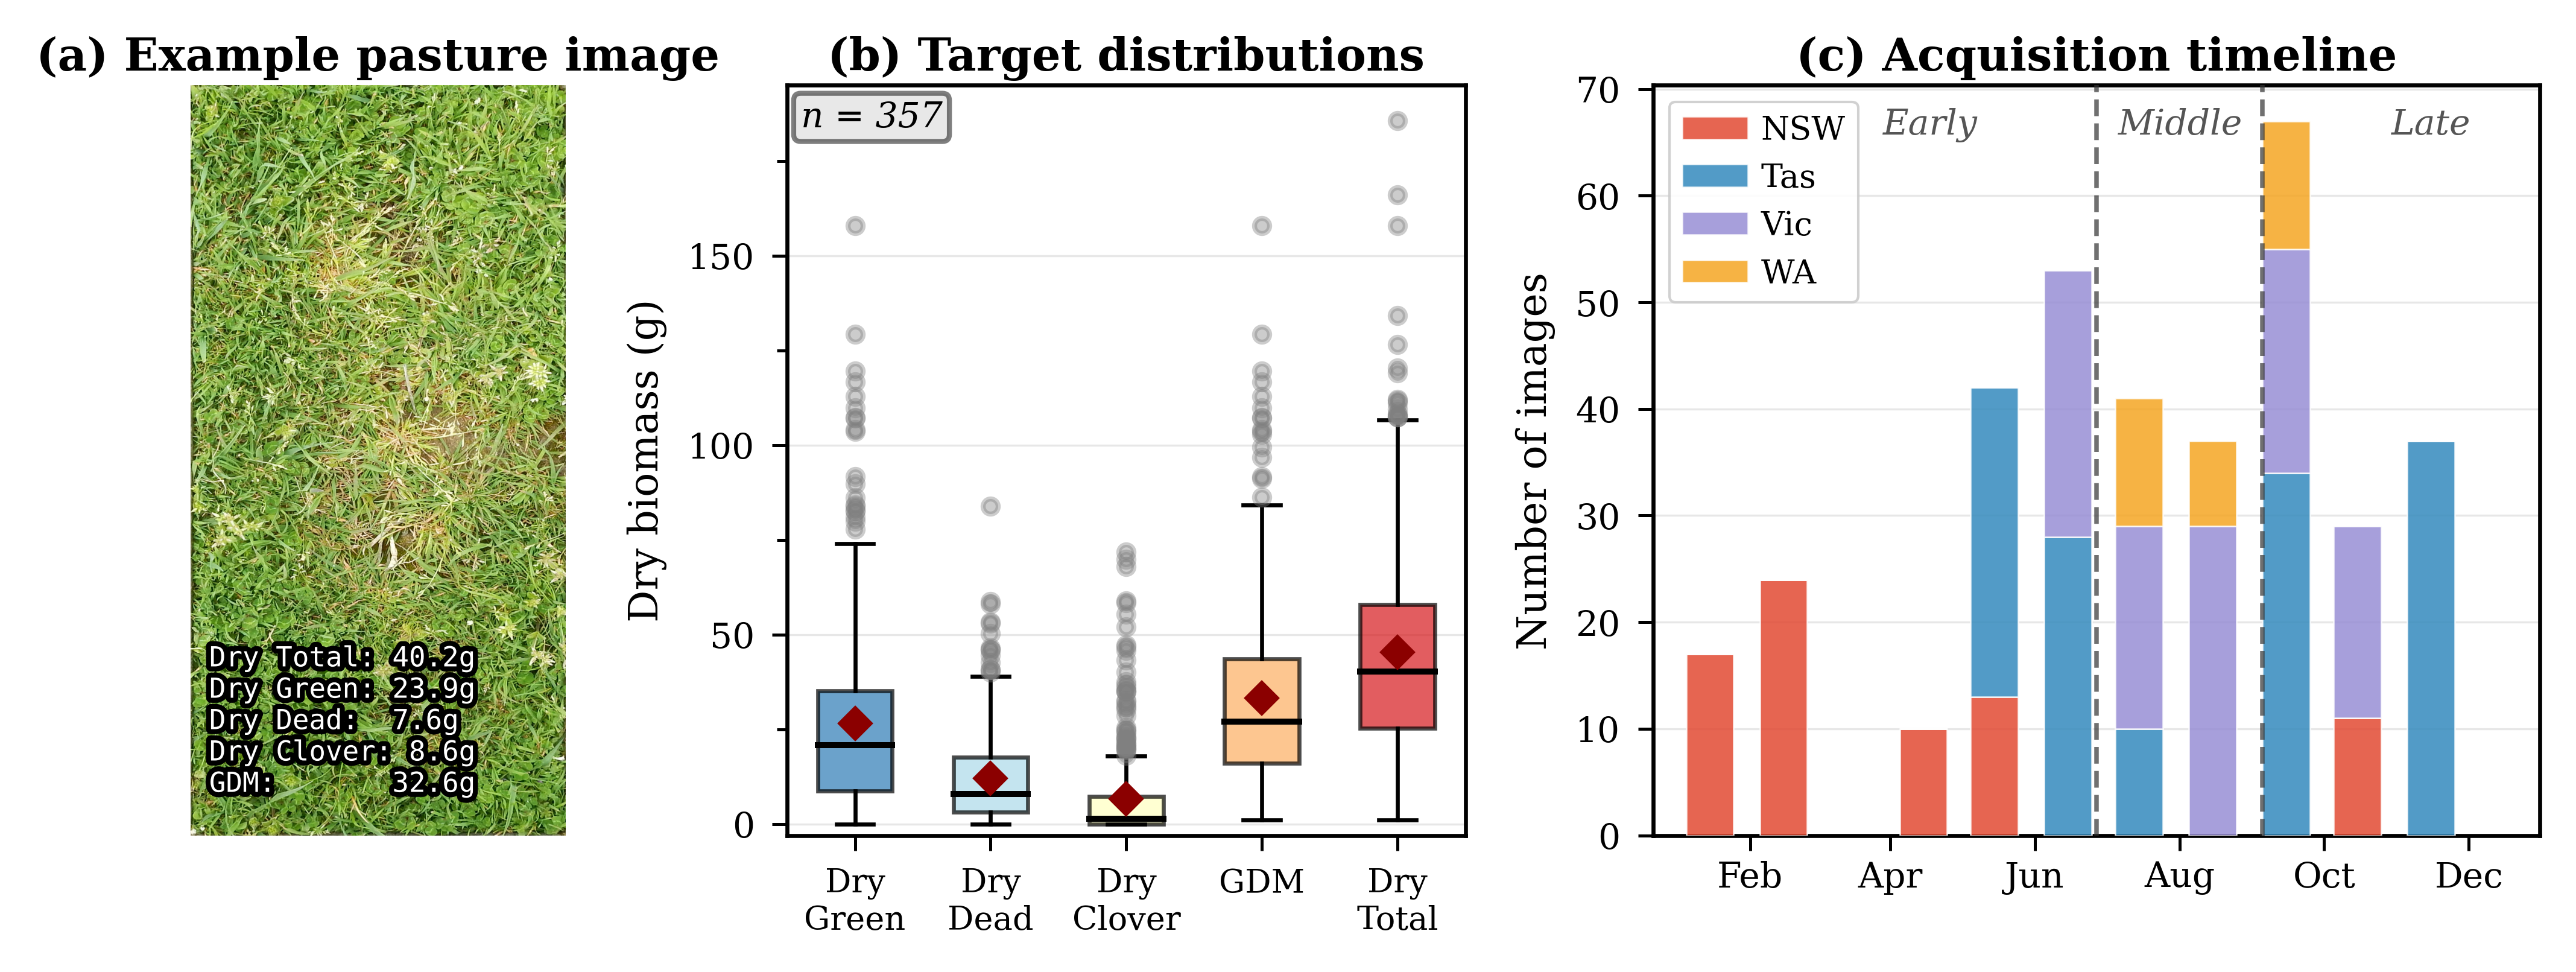
\includegraphics[width=\textwidth]{continut/capitol3/figuri/fig_dataset_overview.png}
%     \caption{
%     Overview of the CSIRO Image2Biomass public split.
%     (a) Example top‑view pasture quadrat (70\,cm $\times$ 30\,cm).
%     (b) Distributions of the five dry‑weight biomass targets ($g$ per quadrat).
%     (c) Temporal distribution of image acquisitions in 2015, coloured by Australian state.
%     Vertical dashed lines indicate the early/middle/late temporal blocks used in the LOPO analysis.
%     }
%     \label{fig:dataset_overview}
% \end{figure*}

% \section{Model Architecture and Training Protocol}

% To exclusively highlight the effect of the validation strategy, the same preprocessing process, the same feature extractor, and the same regression models are used across all experiments, with only the data splitting being varied.

% No target value transformations, prediction reconciliation procedures, or additional post-processing steps are applied, so that the observed differences can be mainly attributed to the validation protocol.

% Each image at $2000{\times}1000$ pixels resolution is split into two halves, left and right, each being resized to $1008{\times}1008$ pixels. During training, spatial augmentations such as horizontal and vertical flips and $90^\circ$ rotations are applied, as well as photometric augmentations of the color jitter type, with parameters: brightness, contrast, saturation $=0.5$, hue $=0.05$.

% These transformations are applied independently to the two image halves, followed by normalization according to ImageNet statistics. During validation, only resizing and normalization are used.

% \subsection{Feature Extraction}

% For visual feature extraction, the DINOv3 ViT-L/16 model \cite{simeoni2025dinov3} was used in frozen mode. For each image half, multiple augmented variants are generated, and each of these is processed by the DINOv3 backbone to produce an embedding of dimension 1024.

% The embeddings from the two image halves are concatenated, resulting in a final feature vector of dimension 2048.

% All embeddings are precomputed and saved to disk, so that the feature extraction process is separated from the training process. During each training iteration, one of the available augmented representations is randomly selected.

% \subsection{The MLP Model}

% For predicting the five target variables, a Multi-Layer Perceptron (MLP) neural network was used, consisting of five independent branches.

% Each branch receives the same feature vector of dimension 2048 as input and produces the prediction for a single biomass component: \textit{Dry\_Total}, \textit{GDM}, \textit{Dry\_Green}, \textit{Dry\_Clover}, and \textit{Dry\_Dead}.

% Each branch consists of three fully connected layers, with hidden dimensions of 1024 and 512 neurons, GELU activations, and dropout with probability $p=0.3$. The last layer is followed by a Softplus function, used to guarantee non-negative predictions.

% \subsection{Training Configuration}

% The model is trained using the AdamW optimizer \cite{loshchilov2017decoupled} with the following parameters: learning rate $1 \times 10^{-3}$, weight decay $1 \times 10^{-2}$, batch size \(8\), for a maximum of \(80\) epochs.

% The loss function used is a weighted mean squared error according to the official competition metric.

% To prevent overfitting, an early stopping mechanism is used based on the local validation metric \(R^2_w\), with a patience of \(15\) epochs.

% \subsection{The Ridge Baseline Model}

% As an additional reference, a Ridge Regression model was also trained using the MultiOutputRegressor class together with RidgeCV.

% It uses the same embedding set and the same validation folds as the MLP model, being evaluated for the values:

% $\{10^{-3},10^{-2},10^{-1},1,10,100,1000\}$

% The purpose of this model is to provide a simple point of comparison and to determine whether the observed effects are generated by the validation protocol or by the complexity of the model used.

% \begin{figure}[t]
%     \centering
%     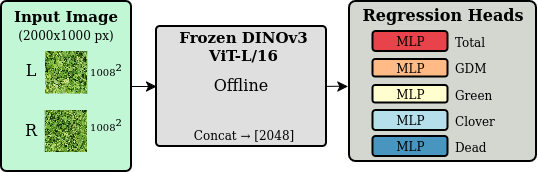
\includegraphics[width=\columnwidth]{continut/capitol3/figuri/fig_pipeline_overview.png}
%     \caption{Overview of the preprocessing, embedding extraction, and multi-branch regression pipeline used in all experiments.}
%     \label{fig:model_overview}
% \end{figure}

% \section{Validation Protocols}

% The purpose of the evaluation is not only to measure local predictive performance, but also to analyze the extent to which different validation protocols reflect the performance obtained on the hidden test set.

% Each 5-fold validation protocol is repeated for five different random seed values. The local results are reported as the mean and standard deviation obtained from these runs.

% For all protocols, stratification is performed using five intervals of the \textit{Dry\_Total} variable, this being the component with the largest weight in the official metric and a relevant indicator of total biomass.

% Three main validation protocols were analyzed:
%     \begin{itemize}
%     \item \textbf{Random CV:} The dataset is split using stratified five-fold cross-validation, without additional constraints regarding the temporal or geographic provenance of the images.
%     \item \textbf{Date CV:} All images collected on the same day are kept together within the same fold. The distribution of data across folds is performed by stratification at the group level.
%     \item \textbf{Date-State CV:} Images that share both the same acquisition date and the same Australian state are considered an indivisible group. The folds are constructed by stratification at the level of these groups.
%     \end{itemize}

% To evaluate how local performances influence the selection of the final model, for each protocol the optimal epoch is calculated as the median of the 25 runs resulting from the combination: $5\text{ folds} \times 5\text{ seeds} = 25$ runs.

% The final model is then retrained from scratch on the entire public dataset using the training duration determined for each protocol.

% During inference, Test Time Augmentation (TTA) is applied using five variants of the imageTheoretical foundation and literature review:

%     \begin{itemize}
%     \item the original image;
%     \item horizontal flip;
%     \item vertical flip;
%     \item $180^\circ$ rotation;
%     \item transpose.
%     \end{itemize}

% The resulting predictions are averaged to generate the final output.

% For each seed, a separate submission is made on the Kaggle platform, and the final performance is calculated as the mean of the scores obtained on the hidden test set.

% As an additional robustness test, the LOPO (Leave-One-Period-Out) procedure was used.

% The data from 2015 was divided into three consecutive temporal blocks:

%     \begin{itemize}
%     \item early period (January 15 – June 26): 130 images;
%     \item middle period (June 29 – September 4): 131 images;
%     \item late period (September 11 – November 10): 96 images.
%     \end{itemize}

% Each period is removed in turn and used exclusively for testing. The LOPO analysis is used solely for exploratory purposes and is not considered a primary evaluation protocol.

% \section{Evaluation Metrics}
% \label{sec:eval}
% \newcommand{\ybar}{\bar{y}_w}

% The main metric used is the global weighted coefficient of determination $R^2_w$, identical to the official metric used in the Kaggle competition.

% Let $\hat{\mathbf{y}} \in \mathbb{R}^{N \times 5}$ be the matrix of predictions generated by the model and $\mathbf{y} \in \mathbb{R}^{N \times 5}$ the matrix of true values. For the five biomass components, the weight vector $\mathbf{w} = [0.1, 0.1, 0.1, 0.2, 0.5]$ is used, corresponding to the variables \textit{Dry\_Green}, \textit{Dry\_Dead}, \textit{Dry\_Clover}, \textit{GDM}, and \textit{Dry\_Total}.

% These weights reflect the relative importance of each component within the official competition metric, with the \textit{Dry\_Total} component having the largest weight.

% In the first step, the global weighted mean is calculated:
% %
% \begin{equation}
%   \ybar = \frac{\sum_{i,j} w_j\, y_{ij}}{\sum_{i,j} w_j},
%   \label{eq:ybar}
% \end{equation}
% %
% Based on this, the residual sum of squares and the total sum of squares are determined:
% %
% \begin{equation}
%   SS_{\text{res}} = \sum_{i,j} w_j\,(y_{ij} - \hat{y}_{ij})^2, \qquad
%   SS_{\text{tot}} = \sum_{i,j} w_j\,(y_{ij} - \ybar)^2,
% \end{equation}
% %
% The weighted coefficient of determination is defined as follows:
% %
% \begin{equation}
%   \boxed{R^2_w = 1 - \frac{SS_{\text{res}}}{SS_{\text{tot}}}}.
% \end{equation}
% %

% In addition to the primary metric $R^2_w$, two classical metrics used in regression problems are also reported: RMSE (Root Mean Squared Error) and MAE (Mean Absolute Error).

% Within the LOPO analysis, the bias for the \textit{Dry\_Total} variable is additionally calculated, to identify possible systematic tendencies of overestimation or underestimation of total biomass.

% To quantify the degree to which a validation protocol overestimates the actual performance on unseen data, an indicator called the optimism gap is defined:

% %
% \begin{equation}
%   \Delta_{\text{hidden}} = R^2_{\text{local}} - R^2_{\text{hidden}},
% \end{equation}
% %

% where $R^2_{\text{local}}$ represents the performance estimated through local validation (calculated using the out-of-fold predictions), and $R^2_{\text{hidden}}$ represents the performance obtained on the competition's hidden test set. Higher values of $\Delta_{\text{hidden}}$ indicate a more pronounced overestimation of the actual performance and, implicitly, a higher degree of optimism of the validation protocol used.